%!TEX root = paper.tex
% Template for PLoS
% Version 1.0 January 2009
%
% To compile to pdf, run:
% latex plos.template
% bibtex plos.template
% latex plos.template
% latex plos.template
% dvipdf plos.template

\documentclass[10pt]{article}
%\documentclass[aps,twocolumn]{revtex4-1}
%\documentclass[aps,twocolumn]{article}
% \usepackage{multicol}

% amsmath package, useful for mathematical formulas
\usepackage{amsmath}
\setcounter{MaxMatrixCols}{50}
% amssymb package, useful for mathematical symbols
\usepackage{amssymb}

% graphicx package, useful for including eps and pdf graphics
% include graphics with the command \includegraphics
\usepackage{graphicx}

% cite package, to clean up citations in the main text. Do not remove.
\usepackage{cite}

\usepackage{color}

% Use doublespacing - comment out for single spacing
%\usepackage{setspace}
%\doublespacing

% Text layout
\topmargin 0.0cm
\oddsidemargin 0.5cm
\evensidemargin 0.5cm
\textwidth 16cm
\textheight 21cm

% Bold the 'Figure #' in the caption and separate it with a period
% Captions will be left justified
\usepackage[labelfont=bf,labelsep=period,justification=raggedright]{caption}

% Remove brackets from numbering in List of References
\makeatletter
\renewcommand{\@biblabel}[1]{\quad#1.}
\makeatother

% Leave date blank
\date{}

\pagestyle{myheadings}
%% ** EDIT HERE **

\usepackage{bussproofs}

% xy-pic for diagrams
\usepackage[all]{xy}
% subcaption
\usepackage{subcaption}
% hyperref
%\usepackage[linkbordercolor={.67 .27 .27},citebordercolor={.09 .29 .54},urlbordercolor={.09 .29 .54}]{hyperref}
\usepackage{hyperref}
\hypersetup{colorlinks=true,
linkcolor=[rgb]{.67 .27 .27},
citecolor=[rgb]{.09 .29 .54},
urlcolor=[rgb]{.09 .29 .54}}

% color table cells http://goo.gl/ZmpJv
\usepackage[table]{xcolor}
% rotate text in table http://goo.gl/Lb4Zd
\usepackage{rotating}
% listings for code highlighting in appendix
\usepackage{listings}
\usepackage{setspace}
%!TEX root = ../plos_template.tex
% http://widerin.org/blog/syntax-highlighting-for-python-scripts-in-latex-documents
\definecolor{Code}{rgb}{0,0,0}
\definecolor{Decorators}{rgb}{0.5,0.5,0.5}
\definecolor{Numbers}{rgb}{0.5,0,0}
\definecolor{MatchingBrackets}{rgb}{0.25,0.5,0.5}
\definecolor{Keywords}{rgb}{.67, .27, .27}
\definecolor{self}{rgb}{0,0,0}
\definecolor{Strings}{rgb}{.09,.29,.54}
\definecolor{Comments}{rgb}{0,0.5,0}
\definecolor{Backquotes}{rgb}{0,0,0}
\definecolor{Classname}{rgb}{0,0,0}
\definecolor{FunctionName}{rgb}{0,0,0}
\definecolor{Operators}{rgb}{0,0,0}
\definecolor{Background}{rgb}{0.98,0.98,0.98}

\lstnewenvironment{python}[1][]{
\lstset{
numbers=left,
numberstyle=\footnotesize,
numbersep=1em,
xleftmargin=1em,
framextopmargin=2em,
framexbottommargin=2em,
showspaces=false,
showtabs=false,
showstringspaces=false,
frame=l,
tabsize=4,
% Basic
basicstyle=\ttfamily\small\setstretch{1},
%basicstyle=\ttfamily\footnotesize,frame=single,#1,
backgroundcolor=\color{Background},
language=Python,
% Comments
commentstyle=\color{Comments}\slshape,
% Strings
stringstyle=\color{Strings},
morecomment=[s][\color{Strings}]{"""}{"""},
morecomment=[s][\color{Strings}]{'''}{'''},
% keywords
morekeywords={import,from,class,def,for,while,if,is,in,elif,else,not,and,or,print,break,continue,return,True,False,None,access,as,,del,except,exec,finally,global,import,lambda,pass,print,raise,try,assert},
keywordstyle={\color{Keywords}\bfseries},
% additional keywords
morekeywords={[2]@invariant},
keywordstyle={[2]\color{Decorators}\slshape},
emph={self},
emphstyle={\color{self}\slshape},
%
}}{}

\usepackage{placeins}
\usepackage{longtable}
\usepackage{dot2texi}
\usepackage{tikz}
\usetikzlibrary{automata,shapes,arrows}
% todo notes see http://www.texample.net/tikz/examples/todo-notes/
\usepackage[colorinlistoftodos]{todonotes}
\usepackage{amsthm}
\usepackage{bibunits}

% hyperref with bibunits
% http://tex.stackexchange.com/a/101495/6784
% \makeatletter
% \def\hyper@natlinkstart#1{%
%   \Hy@backout{#1}%
%   \hyper@linkstart{cite}{cite.\@bibunitname.#1}%
% %                             ^^^^^^^^^^^^^^
%   \def\hyper@nat@current{#1}%
% }

% \def\hyper@natlinkbreak#1#2{%
%   \hyper@linkend#1\hyper@linkstart{cite}{cite.\@bibunitname.#2}%
% %                                             ^^^^^^^^^^^^^^
% }

% \def\hyper@natanchorstart#1{%
%   \hyper@anchorstart{cite.\@bibunitname.#1}%
% %                         ^^^^^^^^^^^^^^
% }

% \def\bibcite#1#2{%
%   \@newl@bel{b}{#1}{\hyper@@link[cite]{}{cite.\@bibunitname.#1}{#2}}%
% %                                             ^^^^^^^^^^^^^^
% }%

% \def\@lbibitem[#1]#2{%
%   \@skiphyperreftrue
%   \H@item[\hyper@anchorstart{cite.\@bibunitname.#2}%
% %                                 ^^^^^^^^^^^^^^
%   \@BIBLABEL{#1}\hyper@anchorend\hfill]%
%   \@skiphyperreffalse
%   \if@filesw
%     \begingroup
%       \let\protect\noexpand
%       \immediate\write\@auxout{%
%         \string\bibcite{#2}{#1}%
%       }%
%     \endgroup
%   \fi
%   \ignorespaces
% }%

% \def\@bibitem#1{%
%   \@skiphyperreftrue\H@item\@skiphyperreffalse
%   \hyper@anchorstart{cite.\@bibunitname.#1}\relax\hyper@anchorend
% %                         ^^^^^^^^^^^^^^
%   \if@filesw
%     \begingroup
%       \let\protect\noexpand
%       \immediate\write\@auxout{%
%         \string\bibcite{#1}{\the\value{\@listctr}}%
%       }%
%     \endgroup
%   \fi
%   \ignorespaces
% }%

% \def\@citex[#1]#2{%
%   \let\@citea\@empty
%   \@cite{%
%     \@for\@citeb:=#2\do{%
%       \@citea
%       \def\@citea{,\penalty\@m\ }%
%       \edef\@citeb{\expandafter\@firstofone\@citeb}%
%       \if@filesw
%         \immediate\write\@auxout{\string\citation{\@citeb}}%
%       \fi
%       \@ifundefined{b@\@citeb}{%
%         \mbox{\reset@font\bfseries ?}%
%         \G@refundefinedtrue
%         \@latex@warning{%
%           Citation `\@citeb' on page \thepage \space undefined%
%         }%
%       }{%
%         \hyper@natlinkstart{#2}%
% %       ^^^^^^^^^^^^^^^^^^^^^^^^
%             \hbox{\csname b@\@citeb\endcsname}%
%         \hyper@natlinkend%
% %       ^^^^^^^^^^^^^^^^^^
%       }%
%     }%
%   }{#1}%
% }%

% \makeatother
% end - hyperref with bibunits

% define colors
\definecolor{DeepRed}{rgb}{.82,.14,.16}
\definecolor{DeepBlue}{rgb}{0,0.36,0.62}

% set depth for table of contents
% http://tex.stackexchange.com/a/17879/6784
% http://tex.stackexchange.com/a/11669/6784
\setcounter{tocdepth}{4}
\setcounter{secnumdepth}{0}

%% ** EDIT HERE **
%% PLEASE INCLUDE ALL MACROS BELOW

\newtheorem{theorem}{Theorem}[section]
\newtheorem{lemma}[theorem]{Lemma}

\theoremstyle{definition}
\newtheorem{definition}[theorem]{Definition}
\newtheorem{example}[theorem]{Example}
\newtheorem{xca}[theorem]{Exercise}

\theoremstyle{remark}
\newtheorem{remark}[theorem]{Remark}


% Set autoref text
% http://tex.stackexchange.com/a/36576/6784
\renewcommand*{\figureautorefname}{Fig.}
\renewcommand*{\equationautorefname}{Eq.}
\renewcommand*{\tableautorefname}{Table}

\renewcommand{\refname}{References}

\newcommand{\beginsupplement}{%
        \setcounter{table}{0}
        \renewcommand{\thetable}{S\arabic{table}}%
        \setcounter{figure}{0}
        \renewcommand{\thefigure}{S\arabic{figure}}%
     }

\def\tr{\mathrm{tr}}
\def\Path{\mathrm{Path}}
\def\hier{\mathbf{Hier}}
\def\Vertex{\mathrm{Vertex}}
\def\adj{\mathrm{adj}}
\def\wprod{\mathbf{wp}}
\def\length{\mathbf{len}}
\def\connectivity{d}
\def\reffigexamplesystemmodules{\ref{fig:modsccsym}A}
\def\reffigscc{\ref{fig:modsccsym}B}
\def\reffighiertransformations{\ref{fig:modsccsym}C}
\def\reffigrobustconnect{\ref{fig:combined}A}
\def\reffigrobusthierarchy{\ref{fig:combined}B}
\def\reffigconnectcycle3D3x3{\ref{fig:combined}C}
\def\reffigconnectdist3D3x3{\ref{fig:combined}D}
%% END MACROS SECTION


\begin{document}

% Add Figure, Table prefixes to references
% http://tex.stackexchange.com/a/6063/6784
\let\ref\autoref

\title{Ensemble Stability of Biological Networks}

\pagenumbering{arabic}

% Title must be 150 characters or less
\begin{center}
{\Large
\textbf{Hierarchical Network Structure Promotes Dynamical Robustness}
}
% Insert Author names, affiliations and corresponding author email.
\\[.5cm]
Cameron Smith$^{1}$,
Raymond S. Puzio$^{1}$,
Aviv Bergman$^{1,2,3,4}$,
\\[.5cm]
$^1$Department of Systems and Computational Biology,\\
$^2$Dominick P. Purpura Department of Neuroscience,\\
$^3$Department of Pathology, Albert Einstein College of Medicine,\\
1301 Morris Park Ave, Bronx, NY 10461, USA\\
$^4$Santa Fe Institute, 1399 Hyde Park Road, Santa Fe, NM 87501, USA
\\[.5cm]
% $\ast$To whom correspondence should be addressed; E-mail: aviv@einstein.yu.edu.
\end{center}

{\begin{quote} \bf
%!TEX root = ../paper.tex
\begin{abstract}
The analysis of dynamical systems that attempts to model chemical reaction, gene-regulatory, population, and ecosystem networks all rely on models having interacting components~\cite{RossCr2003,Alon2006,Palsson2006,HamidBolouri2008,Palsson2011a,Voit2012,Sauro2012}. When the details of these interactions are unknown for biological systems of interest, one effective approach is to study the dynamical properties of an ensemble of models determined by evolutionary constraints that may apply to all such systems~\cite{Gardner1970,May1972,Cohen1984,May1972a,Radius2014}. One such constraint is that of dynamical robustness, the probability of a stable system to remain stable under perturbations to the strength of interactions among its components~\cite{WADDINGTON1942a,Wagner1997,Rutherford1998,VanNimwegen1999,Siegal2002,Bergman2003,Ciliberti2007b,Ciliberti2007,Draghi2010,Wagner2013}. Despite previous investigations, the relationship between dynamical robustness---an important functional characteristic of many biological systems---and network structure is poorly understood. Here we analyze the stability and robustness of a large class of dynamical systems and demonstrate that the most hierarchical network structures, those equivalent to the total ordering, are the most robust. In particular, we determine the probability distribution of robustness over system connectivity and show that robustness is maximized by maximizing the number of links between strongly connected components of the graph representing the underlying system connectivity. We demonstrate that this can be understood in terms of the fact that permutation of strongly connected components is a fundamental symmetry of dynamical robustness, which applies to networks of any number of components and is independent of the distribution from which the strengths of interconnection among components are sampled.  The classification of dynamical robustness based upon a purely topological property provides a fundamental organizing principle that can be used in the context of experimental validation to select among models that break or preserve network hierarchy. This result contributes to an explanation for the observation of hierarchical modularity in biological networks at all scales~\cite{Zhao2006,Ravasz2002,Bhardwaj2010,Colm,Corominas-Murtra2013}.
\end{abstract}

\end{quote}}

% \section{Todo}
% \listoftodos
% \tableofcontents

\section{Introduction}
%!TEX root = ../paper.tex
The traditional approach taken in the study of chemical reaction, gene-regulatory, population, and ecosystem networks is to derive a system of differential equations to model a particular biological network, attempt to fit that model to data and adjust the modeling assumptions along with parameter values until a good fit is achieved \cite{Meyer2014}. All of these models utilize essentially equivalent mathematical structures \ref{fig:biomodelexamples} \cite{RossCr2003,Alon2006,Palsson2006,HamidBolouri2008,Palsson2011a,Voit2012,Sauro2012}. Developing unified mathematical descriptions of all of these is one of the paramount goals of systems biology.

Recent work has demonstrated that as a result of inhomogeneity in the geometry of the sensitivity of the dynamics over the parameter space for such models, this approach allows for a large variety of models to fit the data \cite{Brown2003,Gutenkunst2007,Daniels2008a,Machta2013,Hines2014,Prabakaran2014,Tonsing2014}. In addition, there is often uncertainty about the very structure of such biological networks. In this context, it is crucial to gain insight into what dynamical phenomena are possible to observe within a given class of dynamical systems, which is necessary to understand in order to determine whether or not a particular dynamical phenomenon should be regarded as unique or generic in the development and investigation of models applied to particular systems \cite{Gunawardena2013,Gunawardena2014}. This can be achieved using a method common in statistical physics involving the consideration of an ensemble of systems that, in comparison to one another, appear to have components that are randomly interlinked.

Indeed, investigating generic properties of a large class of dynamical systems was the approach taken by May in models of ecosystem dynamics \cite{Gardner1970,May1972}. The class of dynamical systems studied by May is, however, not restricted to ecosystem dynamics and encompasses, among others, the dynamics of all of the biological networks represented in \ref{fig:biomodelexamples}. May conjectured on the basis of results from random matrix theory what eventually came to be referred to as the May-Wigner stability theorem \cite{Cohen1984,May1972a,Radius2014}, which implies a relationship between a topological property, system connectivity, and a dynamical property, stability.


% The generic applicability of gaining a better understanding of the class of models investigated by May demonstrates the unequivocal value of deeper investigation.  However, work attempting to continue the development of the so-called May-Wigner stability theorem revealed that May's conjectured stability criterion was not as easy to demonstrate as was initially believed.


\section{Results}
%!TEX root = ../paper.tex
Here we determine the relationship between network hierarchy, a topological property, and the probability of \emph{robustness} or \emph{structural stability}, a dynamical property \cite{Smale1967}. Robustness is of interest at all scales of the biological hierarchy, and has been previously studied in the context of gene-regulatory networks \cite{WADDINGTON1942a,VanNimwegen1999,Siegal2002,Ciliberti2007b,Ciliberti2007,Wagner2013}. Intuitively, robustness is the probability of stability to perturbation in the system structure or its parameters for systems which have already been determined to be stable in the sense of linear stability analysis \cite{Davis1962}.

The dynamical model given in terms of a system of differential equations for any network can be represented in terms of an interaction graph (\ref{fig:biomodelexamples} top row). These interaction graphs can be viewed as deriving from the combination of system modules that accept a given pattern of inputs and produce a given pattern of outputs (\reffigexamplesystemmodules). Symmetries are characterized by the ability to interchange these modules or their connectivity without changing some property of the system or its dynamics.

The network architecture can be represented in terms of an adjacency matrix and further abstracted by mapping the interaction graph to the network of strongly connected components (SCCs, see Supplementary Information) (\reffigscc). This map from the interaction graph of a biological network, referred to as $\hier$, has a collection of symmetries shown in \reffighiertransformations. These three symmetries represent transformations that can be performed on the interaction graph that do not change the network of SCCs to which it is associated \reffigscc. Two of these three are also symmetries with respect to dynamical robustness. \ref{fig:robustnesssymmetries} shows an example of these symmetries applied to a specific interaction graph.

We have derived an analytical expression for dynamical robustness as a weighted average of the robustness of the SCCs and the number of links between them that applies to the interaction graph associated to a given dynamical system (Supplementary Material, \ref{eq:sccrobustness}). Examining this expression proves that networks maximizing the number of links between SCCs, will also maximize dynamical robustness (Supplementary Material). This implies that the interaction graphs for systems that are the most robust will also maximize the overall number of SCCs. This analytical result predicts that any biological network whose associated dynamical system has the interaction graph \reffigscc $\,$ top will be more robust than those associated to any of the other interaction graphs in \reffigscc. Because this result is purely topological in nature, it does not depend at all upon any particular details such as the probability distribution from which the component interaction strengths are sampled or the size of the system. The result that dynamical robustness is correlated with system hierarchy therefore applies to an even broader class of dynamical systems than the particular random ensembles we have studied directly.

To test this prediction, we computed the probability distribution of stability and dynamical robustness relative to biological network architecture for ensembles of systems having two or three interacting components (see \ref{tab:structstabmat} and \ref{tab:structstabmat3}). For all of these, we found that robustness is correlated with connectivity, but that the most robust systems have intermediate connectivity for a given network size (\reffigrobustconnect). Accounting for the number of cycles in a network architecture reveals a strong correlation between robustness and connectivity that was hidden when networks with any number of cycles were considered together (\reffigconnectcycle3D3x3). While the most hierarchical network architecture will always lack cycles altogether, cycle number alone is clearly insufficient to account for robustness as the members of each class span nearly the entire range of possible robustness values. Consistent with our analysis of the symmetries of robustness, we found that the most hierarchical network architecture is the most robust (\reffigrobusthierarchy). Moreover, if we consider hierarchy partitioned by connectivity, we find that there is a monotonic increase in robustness following any line of increasing hierarchy in \reffigconnectdist3D3x3.

% \textcolor{red}{We precisely compute the probability of stability and the robustness as a distribution over system connectivity for all systems containing two or three interacting components. We find that stability to structural perturbations of this class of dynamical systems is correlated with connectivity, number of cycles, and the number of links between strongly connected components (SCCs) of the underlying interdependency graph. The latter correlation derives from the fact that the permutation of SCCs is a symmetry of dynamical robustness.}


\section{Discussion}
%!TEX root = ../paper.tex
% Our development suggests two predictions that could be used to test the theory described here. One is that,
Our theory predicts that any ensemble of systems where robustness has been positively selected over a sufficiently long period of time should exhibit a bias toward more hierarchical network topologies. For example, at the ecological level, a system subjected to the environmental stress of overfishing, which may imply selection for robustness, has been observed to exhibit such a bias toward more hierarchical network architectures \cite{Bascompte2005}. In the short term, this prediction may be further evaluated at the levels of both metabolic and transcription factor networks, which have already been shown to display hierarchical structure, but whose dynamics have not been sufficiently well characterized to ascertain their robustness \cite{Zhao2006,Bhardwaj2010,Colm}.
%The other prediction of the theory outlined here that may be able to be checked is the converse statement that an ensemble of systems demonstrating a positive or negative bias in their network topology toward hierarchy may have been under selection for, or respectively against, robustness. Of course, in this case, factors other than selection for robustness would not be ruled out by this analysis alone.
In the long term, this prediction may be evaluated using experimental evolution by comparing the degree of hierarchy that emerges in the evolution of gene regulatory network topology in the context of both static and fluctuating environments that differentially select for robustness \cite{Leroi1994}.

%The fact that such a relationship exists has the potential to unify our understanding of biological networks.
In order to further this work from a theoretical perspective, it will be necessary to deepen our understanding of the relationship between dynamical robustness and the underlying network topology.
%One approach is to attempt to compute robustness for systems of larger size. Using existing methods, this would require large-scale Monte Carlo simulations. However,
It may be possible to prove a bound on the robustness of individual SCCs, which could provide more definite knowledge and circumvent the need for expensive simulations. The conservation of robustness with respect to nontrivial symmetries including the interchange of SCCs and permutation within SCCs suggests the existence of an evolutionary neutral space. A deeper mathematical characterization of the full symmetry groupoid of dynamical robustness may thus help to characterize this potential evolutionary constraint \cite{Golubitsky2006}.

The relationship between structure and function is fundamental to networks at every level of the biological hierarchy. Equally fundamental is the ability of systems to persist over long periods of time, which is dependent upon their dynamical robustness. Here we have demonstrated a structure-function relationship wherein biological networks that are more hierarchical are more robust and thus more likely to persist in the evolutionary process.
%Moreover, this result is formulated at a level of abstraction that allows its conclusions to apply independently to each of these levels.


\section{Acknowlegements}  The authors would like to thank Jay Sulzberger and Ximo Pechuan for useful suggestions and discussions.

\pagebreak

\bibliographystyle{pnas}
\bibliography{bib/books,bib/papers}

\pagebreak
\FloatBarrier

\section{Figure Legends}
%!TEX root = ../paper.tex

% \begin{figure}[!ht]
% \centering
% \noindent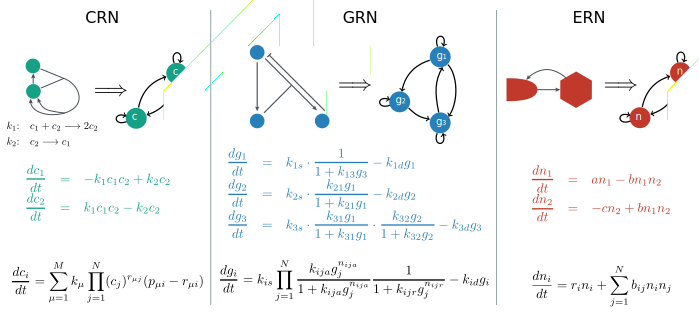
\includegraphics[width=0.9\columnwidth]{fig/biomodelexamples.pdf}
% \caption{{\bf Dynamical models in systems biology.} The top row represents a chemical reaction network (CRN) \cite{Shinar2010}, a gene regulatory network (GRN) \cite{Karlebach2008}, and an ecological regulatory network (ERN) \cite{Rohr2014} in terms of the graphical methods specific to each field mapped into the interaction graph, which provides a unified representation for networks across these fields. The second row represents a particular example of a system of differential equations that are used to model a biological network within each of the domains of application considered here. The third row shows the general form of a system of differential equations that can be used to model any network architecture within each domain.}
% \label{fig:biomodelexamples}
% \end{figure}

% \pagebreak

% \begin{figure}[!ht]
% \centering
% \noindent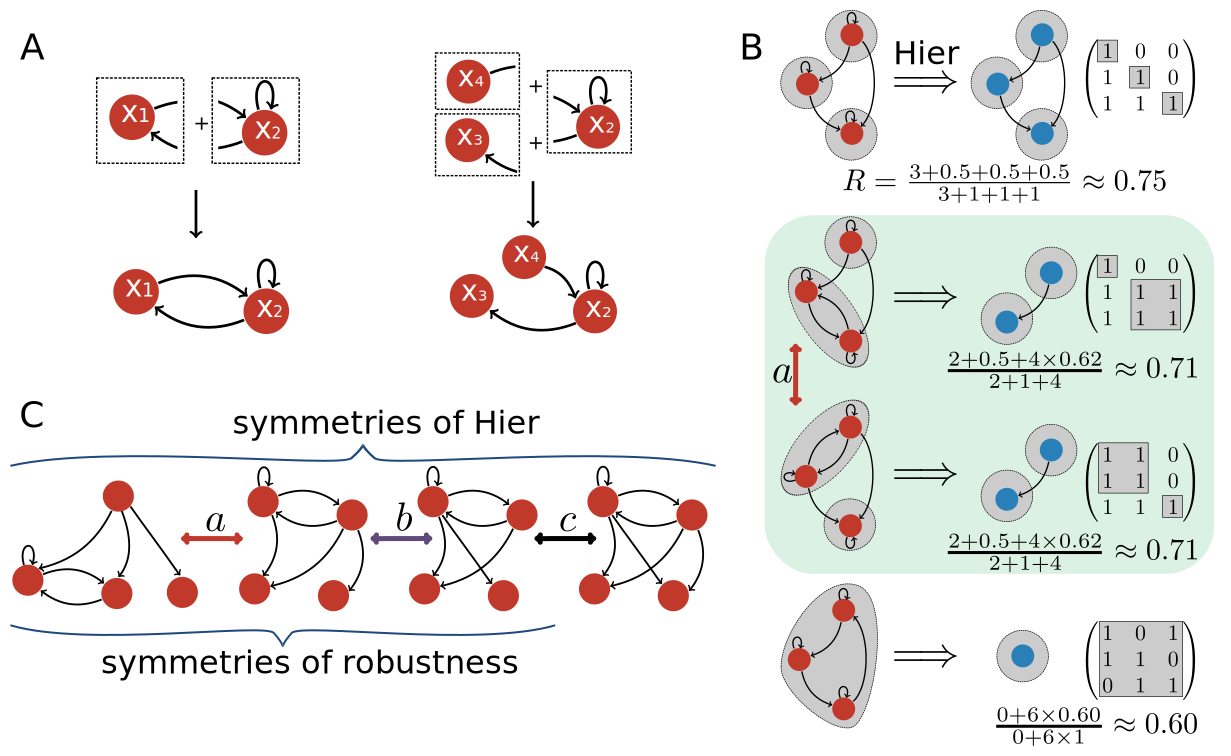
\includegraphics[width=0.9\columnwidth]{fig/modsccsym.pdf}
% \caption{{\bf Open systems, strongly connected components and symmetries of robustness.} (A) Example of the combination of open system modules to construct closed systems. (B) SCCs highlighted in gray for each of the four graphs representing the interdependencies relevant to four different three variable systems. The most hierarchical network, top panel, is the one that maximizes the number of SCCs and the number of links between them. We therefore define hierarchy as $max(\hbox{ED}) - \hbox{ED}$ where ED is the edit distance representing the number of link addition/deletion operations necessary to transform a given graph into the most hierarchical one. The two panels in the middle represent examples of hierarchical modular systems that posess both modularity (i.e. SCCs with more than one variable) and hierarchy. (C) Symmetries of the $\hier$ transformation between graphs and SCCs. The transformation $a$ represents an interchange of SCCs, $b$ moving a link between nodes in a component and $c$ adding a link. All three transformations represent symmetries of the $\hier$ transformation from graphs to SCCs while only $a$ and $b$ are symmetries of robustness.}
% \label{fig:modsccsym}
% \end{figure}

% \pagebreak


% \begin{figure}[!ht]
% \centering
% \noindent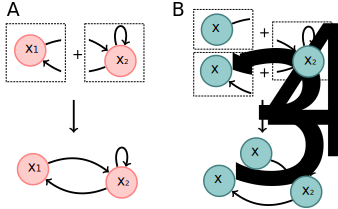
\includegraphics[width=0.4\columnwidth]{fig/examplesystemmodules.pdf}
% \caption{{\bf Example of the combination of open system modules to construct closed systems.} (A) Example of combining two open modules to construct a closed system of two components (B) Analogous example for combining three open modules to construct a closed system with three components}
% \label{fig:examplesystemmodules}
% \end{figure}

% \pagebreak

% \begin{figure}[!ht]
% \centering
% \noindent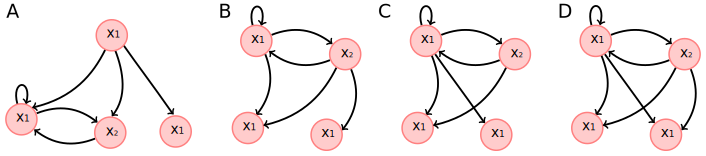
\includegraphics[width=0.7\columnwidth]{fig/hiertransformations.pdf}
% \caption{{\bf Symmetries of the $\hier$ transformation between graphs and SCCs.} The transformation A represents an interchange of SCCs, B moving a link between nodes in a component and C adding a link. All three transformations represent symmetries of the $\hier$ transformation from graphs to SCCs while only A and B are symmetries of robustness.}
% \label{fig:hiertransformations}
% \end{figure}

% \pagebreak

% \begin{figure}[!ht]
% \centering
% \noindent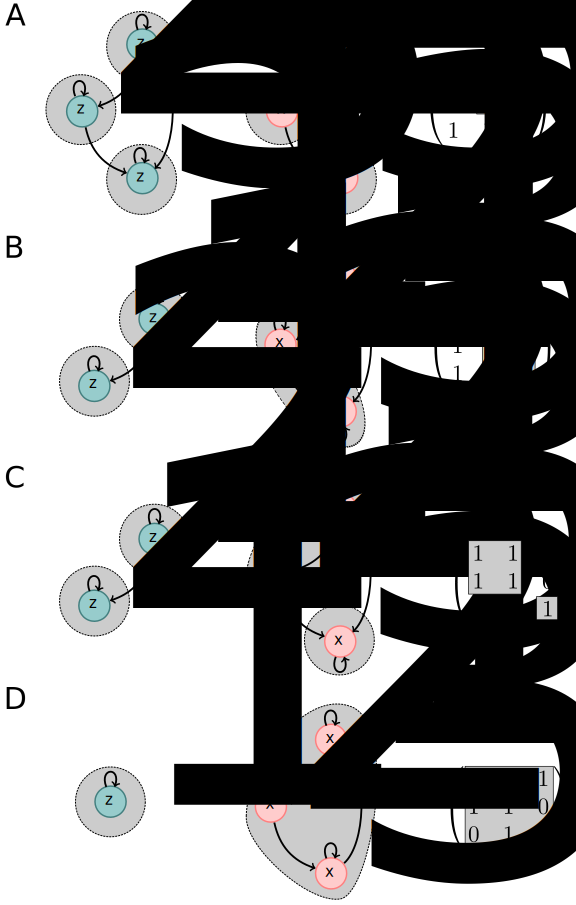
\includegraphics[width=0.4\columnwidth]{fig/scc2.pdf}
% \caption{{\bf Example of strongly connected components.} (A) - (D) show strongly connected components highlighted in gray for each of the four graphs representing the interdependencies relevant to four different three variable systems. Note that the most hierarchical system in (A) has the highest possible number of connected components, three, whereas the system containing a single cycle and therefore posessing no hierarchy contains only one connected component. Systems (B) and (C) represent examples of hierarchical modular systems that posess both modularity and hierarchy.}
% \label{fig:scc}
% \end{figure}

% \pagebreak

% \begin{figure}[!ht]
% \centering
% \noindent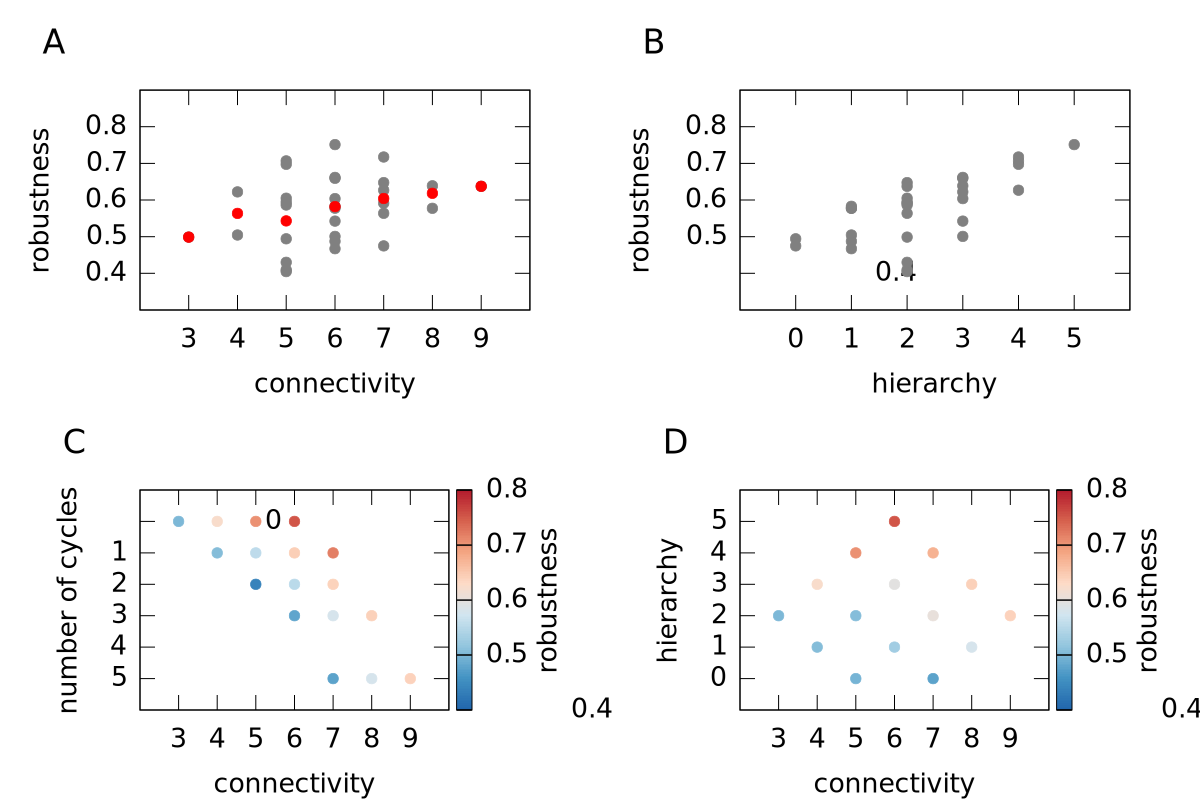
\includegraphics[width=1.0\columnwidth]{fig/combinedfigs.pdf}
% \caption{{\bf Characterization of stability and robustness according to properties of system structure for three variable systems} (A) Robustness versus connectivity. The red line represents a best fit in the least-squares sense with Pearson product-moment correlation coefficient $r=0.29$. The lowest and highest robustness network architectures are labelled. Other network architectures are shown in \ref{tab:structstabmat3}. (B) Robustness versus hierarchy. Correlation coefficient $r=0.67$. (C) Number of cycles and (D) hierarchy vs connectivity and robustness. The color of each point represents the average robustness of all graphs having the parameters specified on the $x$ and $y$ axes.
% }
% \label{fig:combined}
% \end{figure}

% \pagebreak

% \begin{figure}[!ht]
% \centering
% \noindent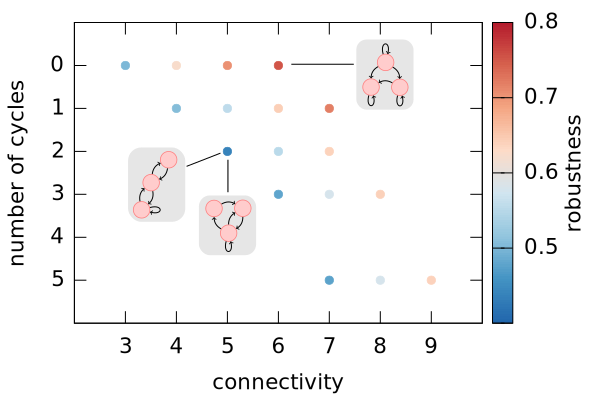
\includegraphics[width=0.8\columnwidth]{fig/connectcycle3D3x3.pdf}
% \caption{{\bf Robustness versus number of cycles and connectivity for three variable systems.} Each point represents the average robustness of all graphs having a given number of cycles and connectivity.}
% \label{fig:connectcycle3D3x3}
% \end{figure}

% \pagebreak

% \begin{figure}[!ht]
% \centering
% \noindent\includegraphics[width=0.8\columnwidth]{fig/connectdist3D3x3.pdf}
% \caption{{\bf Robustness versus hierarchy and connectivity for three variable systems.} Each point represents the average robustness of all graphs having a given hierarchy and connectivity.}
% \label{fig:connectdist3D3x3}
% \end{figure}



\pagebreak
\FloatBarrier

\beginsupplement
\setcounter{secnumdepth}{4}
\section{Supplementary Material}

\input{tex/supplement}
\pagebreak

%!TEX root = ../paper.tex
% \begin{figure}[!ht]
% \centering
% \noindent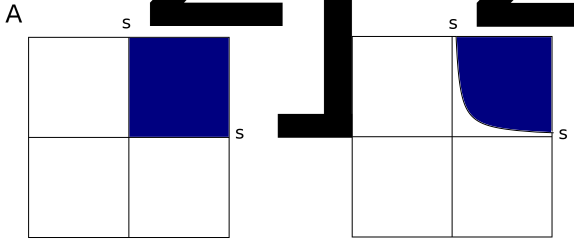
\includegraphics[width=0.7\columnwidth]{fig/region2and3.pdf}
% \caption{{\bf Stability conditions on coefficients of the characteristic polynomial for two and three component systems.} The regions correspond to all possible relationships between the invariants determined by the characteristic polynomial.}
% \label{fig:region2and3}
% \end{figure}

% \pagebreak

% \begin{figure}[!ht]
% \centering
% \noindent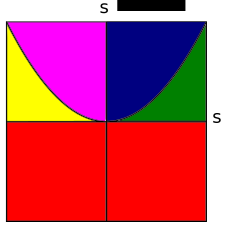
\includegraphics[width=0.5\columnwidth]{fig/region2x2.pdf}
% \caption{{\bf Stability conditions on coefficients of the characteristic polynomial for two component systems.} The regions correspond to all possible relationships between the invariants determined by the characteristic polynomial. Colors correspond to the regions given in the main text Green: $R_{2000}$, Red: $R_{1100}$, Yellow: $R_{0200}$, Magenta: $R_{0002}$, Blue: $R_{0020}$.}
% \label{fig:region2x2}
% \end{figure}

% \pagebreak

% \begin{figure}[!ht]
% \centering
% \noindent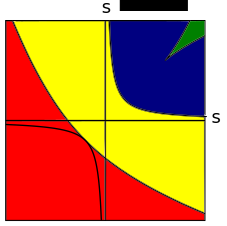
\includegraphics[width=0.5\columnwidth]{fig/region3x3.pdf}
% \caption{{\bf Stability conditions on coefficients of the characteristic polynomial for three component systems.} Colors correspond to the following regions Green: $R_{3000}$, Red: $R_{1200}$, Yellow: $R_{1002}$, Blue: $R_{1020}$. This is the plane $s_3=1$.}
% \label{fig:region3x3}
% \end{figure}

\pagebreak

% \section{Tables}
% \todo{Fill out notation table}
% %!TEX root = ../paper.tex
\begin{table}[h]
\begin{center}
\begin{tabular}{ c || c }
\hline
symbol & interpretation\\
\hline
$\connectivity$ & connectivity\\
\end{tabular}
\end{center}
\caption{{\bf Table of notation}.}\label{tab:notation}
\end{table}

%!TEX root = ../paper.tex
\newcommand{\specialcell}[2][c]{%
  \begin{tabular}[#1]{@{}c@{}}#2\end{tabular}}

\begin{table}[h]
\begin{center}
\begin{tabular}{ c || c | c | c }
\hline
matrix & connectivity & \specialcell{probability of stability\\to perturbation} & \specialcell{probability\\of stability}\\
\hline
  $\begin{pmatrix}
a & b \\
d & c
\end{pmatrix}$ & 4 & 0.62 & 0.25 \\
  $\begin{pmatrix}
a & b \\
d & 0
\end{pmatrix}$, $\begin{pmatrix}
0 & b \\
d & c
\end{pmatrix}$ & 3 & 0.5 & 0.25 \\
  $\begin{pmatrix}
a & 0 \\
d & c
\end{pmatrix}$, $\begin{pmatrix}
a & b \\
0 & c
\end{pmatrix}$ & 3 & 0.67 & 0.25 \\
$\begin{pmatrix}
a & 0 \\
0 & c
\end{pmatrix}$ & 2 & 0.5 & 0.25 \\
\end{tabular}
\end{center}
\caption{{\bf Probability of stability under resampling and \emph{a priori} stability for two component systems derived analytically}. All matrices not listed have $0$ probability of stability.}\label{tab:structstabmat}
\end{table}

\pagebreak
%!TEX root = ../paper.tex
\begin{longtable}{ c | c || c | c | c | c | c }
\hline
matrix & \specialcell{orbit\\size} & connectivity & \specialcell{edit\\distance} & \specialcell{cycle\\number} & \specialcell{probability of stability\\to perturbation} & \specialcell{probability\\of stability}\\
\hline
$\begin{pmatrix}
1 & 0 & 0\\
0 & 1 & 0\\
0 & 0 & 1\\
\end{pmatrix}$ & 1 & 3 & 3 & 0 & 0.499 & 0.126\\
$\begin{pmatrix}
0 & 0 & 1\\
0 & 1 & 0\\
1 & 0 & 1\\
\end{pmatrix}$ & 6 & 4 & 4 & 1 & 0.505 & 0.121\\
$\begin{pmatrix}
1 & 0 & 0\\
0 & 1 & 1\\
0 & 0 & 1\\
\end{pmatrix}$ & 6 & 4 & 2 & 0 & 0.622 & 0.127\\
$\begin{pmatrix}
0 & 0 & 1\\
0 & 1 & 1\\
1 & 0 & 1\\
\end{pmatrix}$ & 12 & 5 & 3 & 1 & 0.595 & 0.121\\
$\begin{pmatrix}
0 & 0 & 1\\
0 & 1 & 1\\
1 & 1 & 0\\
\end{pmatrix}$ & 6 & 5 & 5 & 2 & 0.494 & 0.128\\
$\begin{pmatrix}
0 & 1 & 1\\
0 & 0 & 1\\
1 & 0 & 1\\
\end{pmatrix}$ & 12 & 5 & 3 & 2 & 0.41 & 0.061\\
$\begin{pmatrix}
0 & 1 & 0\\
0 & 1 & 1\\
1 & 0 & 1\\
\end{pmatrix}$ & 6 & 5 & 3 & 1 & 0.43 & 0.078\\
$\begin{pmatrix}
0 & 1 & 1\\
0 & 1 & 0\\
1 & 0 & 1\\
\end{pmatrix}$ & 12 & 5 & 3 & 1 & 0.605 & 0.12\\
$\begin{pmatrix}
0 & 1 & 1\\
0 & 1 & 1\\
1 & 0 & 0\\
\end{pmatrix}$ & 6 & 5 & 3 & 2 & 0.405 & 0.06\\
$\begin{pmatrix}
1 & 0 & 1\\
0 & 1 & 1\\
0 & 0 & 1\\
\end{pmatrix}$ & 6 & 5 & 1 & 0 & 0.698 & 0.122\\
$\begin{pmatrix}
1 & 0 & 0\\
0 & 1 & 1\\
0 & 1 & 1\\
\end{pmatrix}$ & 3 & 5 & 3 & 1 & 0.587 & 0.128\\
$\begin{pmatrix}
1 & 0 & 1\\
0 & 1 & 0\\
0 & 1 & 1\\
\end{pmatrix}$ & 6 & 5 & 1 & 0 & 0.707 & 0.127\\
$\begin{pmatrix}
0 & 0 & 1\\
0 & 1 & 1\\
1 & 1 & 1\\
\end{pmatrix}$ & 6 & 6 & 4 & 2 & 0.578 & 0.121\\
$\begin{pmatrix}
0 & 1 & 1\\
0 & 0 & 1\\
1 & 1 & 1\\
\end{pmatrix}$ & 6 & 6 & 4 & 3 & 0.487 & 0.081\\
$\begin{pmatrix}
0 & 1 & 1\\
0 & 1 & 1\\
1 & 0 & 1\\
\end{pmatrix}$ & 12 & 6 & 2 & 2 & 0.543 & 0.098\\
$\begin{pmatrix}
0 & 1 & 0\\
0 & 1 & 1\\
1 & 1 & 1\\
\end{pmatrix}$ & 6 & 6 & 2 & 2 & 0.501 & 0.088\\
$\begin{pmatrix}
0 & 1 & 1\\
0 & 1 & 0\\
1 & 1 & 1\\
\end{pmatrix}$ & 12 & 6 & 2 & 1 & 0.662 & 0.123\\
$\begin{pmatrix}
0 & 1 & 1\\
0 & 1 & 1\\
1 & 1 & 0\\
\end{pmatrix}$ & 12 & 6 & 4 & 3 & 0.467 & 0.079\\
$\begin{pmatrix}
0 & 1 & 1\\
1 & 1 & 0\\
1 & 0 & 1\\
\end{pmatrix}$ & 3 & 6 & 4 & 2 & 0.583 & 0.13\\
$\begin{pmatrix}
1 & 0 & 1\\
0 & 1 & 1\\
0 & 1 & 1\\
\end{pmatrix}$ & 12 & 6 & 2 & 1 & 0.659 & 0.124\\
$\begin{pmatrix}
1 & 1 & 1\\
0 & 1 & 1\\
0 & 0 & 1\\
\end{pmatrix}$ & 6 & 6 & 0 & 0 & 0.751 & 0.124\\
$\begin{pmatrix}
1 & 1 & 0\\
0 & 1 & 1\\
1 & 0 & 1\\
\end{pmatrix}$ & 2 & 6 & 2 & 1 & 0.604 & 0.097\\
$\begin{pmatrix}
0 & 1 & 1\\
0 & 1 & 1\\
1 & 1 & 1\\
\end{pmatrix}$ & 12 & 7 & 3 & 3 & 0.564 & 0.103\\
$\begin{pmatrix}
0 & 1 & 1\\
1 & 0 & 1\\
1 & 1 & 1\\
\end{pmatrix}$ & 3 & 7 & 5 & 5 & 0.475 & 0.068\\
$\begin{pmatrix}
0 & 1 & 1\\
1 & 1 & 1\\
1 & 0 & 1\\
\end{pmatrix}$ & 6 & 7 & 3 & 3 & 0.591 & 0.108\\
$\begin{pmatrix}
1 & 1 & 1\\
0 & 1 & 1\\
0 & 1 & 1\\
\end{pmatrix}$ & 6 & 7 & 1 & 1 & 0.717 & 0.119\\
$\begin{pmatrix}
1 & 0 & 1\\
0 & 1 & 1\\
1 & 1 & 1\\
\end{pmatrix}$ & 3 & 7 & 3 & 2 & 0.648 & 0.122\\
$\begin{pmatrix}
1 & 1 & 1\\
0 & 1 & 1\\
1 & 0 & 1\\
\end{pmatrix}$ & 6 & 7 & 1 & 2 & 0.627 & 0.105\\
$\begin{pmatrix}
0 & 1 & 1\\
1 & 1 & 1\\
1 & 1 & 1\\
\end{pmatrix}$ & 3 & 8 & 4 & 5 & 0.577 & 0.093\\
$\begin{pmatrix}
1 & 1 & 1\\
0 & 1 & 1\\
1 & 1 & 1\\
\end{pmatrix}$ & 6 & 8 & 2 & 3 & 0.639 & 0.109\\
$\begin{pmatrix}
1 & 1 & 1\\
1 & 1 & 1\\
1 & 1 & 1\\
\end{pmatrix}$ & 1 & 9 & 3 & 5 & 0.638 & 0.106\\
\caption{{\bf Robustness and stability for three variable systems estimated via Monte Carlo sampling.} All matrices not listed have $0$ probability of stability.}\label{tab:structstabmat3}
\end{longtable}


% %!TEX root = ../paper.tex
% \onecolumn
\begin{longtable*}{ c || c | c | c | c }
\hline
matrix & connectivity & cycle number & \specialcell{probability of stability\\to perturbation} & probability of stability\\
\hline
\begin{tikzpicture}[scale=0.6,
every state/.style={draw=red!50,very thick,fill=red!20}]
\begin{dot2tex}[styleonly,codeonly,neato,mathmode]
digraph G {
d2ttikzedgelabels = true;
node [style="state"];
edge [lblstyle="auto",topath="bend left",style="line width=1.5pt"];
1 -> 1 [topath="loop above"];
2 -> 2 [topath="loop above"];
3 -> 3 [topath="loop above"];
}
\end{dot2tex}
\end{tikzpicture} & 3 & 0 & 0.499 & 0.126\\
\begin{tikzpicture}[scale=0.6,
every state/.style={draw=red!50,very thick,fill=red!20}]
\begin{dot2tex}[styleonly,codeonly,neato,mathmode]
digraph G {
d2ttikzedgelabels = true;
node [style="state"];
edge [lblstyle="auto",topath="bend left",style="line width=1.5pt"];
3 -> 1;
2 -> 2 [topath="loop above"];
1 -> 3;
3 -> 3 [topath="loop above"];
}
\end{dot2tex}
\end{tikzpicture} & 4 & 1 & 0.505 & 0.121\\
\begin{tikzpicture}[scale=0.6,
every state/.style={draw=red!50,very thick,fill=red!20}]
\begin{dot2tex}[styleonly,codeonly,neato,mathmode]
digraph G {
d2ttikzedgelabels = true;
node [style="state"];
edge [lblstyle="auto",topath="bend left",style="line width=1.5pt"];
1 -> 1 [topath="loop above"];
2 -> 2 [topath="loop above"];
3 -> 2;
3 -> 3 [topath="loop above"];
}
\end{dot2tex}
\end{tikzpicture} & 4 & 0 & 0.622 & 0.127\\
\begin{tikzpicture}[scale=0.6,
every state/.style={draw=red!50,very thick,fill=red!20}]
\begin{dot2tex}[styleonly,codeonly,neato,mathmode]
digraph G {
d2ttikzedgelabels = true;
node [style="state"];
edge [lblstyle="auto",topath="bend left",style="line width=1.5pt"];
3 -> 1;
2 -> 2 [topath="loop above"];
3 -> 2;
1 -> 3;
3 -> 3 [topath="loop above"];
}
\end{dot2tex}
\end{tikzpicture} & 5 & 1 & 0.595 & 0.121\\
\begin{tikzpicture}[scale=0.6,
every state/.style={draw=red!50,very thick,fill=red!20}]
\begin{dot2tex}[styleonly,codeonly,neato,mathmode]
digraph G {
d2ttikzedgelabels = true;
node [style="state"];
edge [lblstyle="auto",topath="bend left",style="line width=1.5pt"];
3 -> 1;
2 -> 2 [topath="loop above"];
3 -> 2;
1 -> 3;
2 -> 3;
}
\end{dot2tex}
\end{tikzpicture} & 5 & 2 & 0.494 & 0.128\\
\begin{tikzpicture}[scale=0.6,
every state/.style={draw=red!50,very thick,fill=red!20}]
\begin{dot2tex}[styleonly,codeonly,neato,mathmode]
digraph G {
d2ttikzedgelabels = true;
node [style="state"];
edge [lblstyle="auto",topath="bend left",style="line width=1.5pt"];
2 -> 1;
3 -> 1;
3 -> 2;
1 -> 3;
3 -> 3 [topath="loop above"];
}
\end{dot2tex}
\end{tikzpicture} & 5 & 2 & 0.41 & 0.061\\
\begin{tikzpicture}[scale=0.6,
every state/.style={draw=red!50,very thick,fill=red!20}]
\begin{dot2tex}[styleonly,codeonly,neato,mathmode]
digraph G {
d2ttikzedgelabels = true;
node [style="state"];
edge [lblstyle="auto",topath="bend left",style="line width=1.5pt"];
2 -> 1;
2 -> 2 [topath="loop above"];
3 -> 2;
1 -> 3;
3 -> 3 [topath="loop above"];
}
\end{dot2tex}
\end{tikzpicture} & 5 & 1 & 0.43 & 0.078\\
\begin{tikzpicture}[scale=0.6,
every state/.style={draw=red!50,very thick,fill=red!20}]
\begin{dot2tex}[styleonly,codeonly,neato,mathmode]
digraph G {
d2ttikzedgelabels = true;
node [style="state"];
edge [lblstyle="auto",topath="bend left",style="line width=1.5pt"];
2 -> 1;
3 -> 1;
2 -> 2 [topath="loop above"];
1 -> 3;
3 -> 3 [topath="loop above"];
}
\end{dot2tex}
\end{tikzpicture} & 5 & 1 & 0.605 & 0.12\\
\begin{tikzpicture}[scale=0.6,
every state/.style={draw=red!50,very thick,fill=red!20}]
\begin{dot2tex}[styleonly,codeonly,neato,mathmode]
digraph G {
d2ttikzedgelabels = true;
node [style="state"];
edge [lblstyle="auto",topath="bend left",style="line width=1.5pt"];
2 -> 1;
3 -> 1;
2 -> 2 [topath="loop above"];
3 -> 2;
1 -> 3;
}
\end{dot2tex}
\end{tikzpicture} & 5 & 2 & 0.405 & 0.06\\
\begin{tikzpicture}[scale=0.6,
every state/.style={draw=red!50,very thick,fill=red!20}]
\begin{dot2tex}[styleonly,codeonly,neato,mathmode]
digraph G {
d2ttikzedgelabels = true;
node [style="state"];
edge [lblstyle="auto",topath="bend left",style="line width=1.5pt"];
1 -> 1 [topath="loop above"];
3 -> 1;
2 -> 2 [topath="loop above"];
3 -> 2;
3 -> 3 [topath="loop above"];
}
\end{dot2tex}
\end{tikzpicture} & 5 & 0 & 0.698 & 0.122\\
\begin{tikzpicture}[scale=0.6,
every state/.style={draw=red!50,very thick,fill=red!20}]
\begin{dot2tex}[styleonly,codeonly,neato,mathmode]
digraph G {
d2ttikzedgelabels = true;
node [style="state"];
edge [lblstyle="auto",topath="bend left",style="line width=1.5pt"];
1 -> 1 [topath="loop above"];
2 -> 2 [topath="loop above"];
3 -> 2;
2 -> 3;
3 -> 3 [topath="loop above"];
}
\end{dot2tex}
\end{tikzpicture} & 5 & 1 & 0.587 & 0.128\\
\begin{tikzpicture}[scale=0.6,
every state/.style={draw=red!50,very thick,fill=red!20}]
\begin{dot2tex}[styleonly,codeonly,neato,mathmode]
digraph G {
d2ttikzedgelabels = true;
node [style="state"];
edge [lblstyle="auto",topath="bend left",style="line width=1.5pt"];
1 -> 1 [topath="loop above"];
3 -> 1;
2 -> 2 [topath="loop above"];
2 -> 3;
3 -> 3 [topath="loop above"];
}
\end{dot2tex}
\end{tikzpicture} & 5 & 0 & 0.707 & 0.127\\
\begin{tikzpicture}[scale=0.6,
every state/.style={draw=red!50,very thick,fill=red!20}]
\begin{dot2tex}[styleonly,codeonly,neato,mathmode]
digraph G {
d2ttikzedgelabels = true;
node [style="state"];
edge [lblstyle="auto",topath="bend left",style="line width=1.5pt"];
3 -> 1;
2 -> 2 [topath="loop above"];
3 -> 2;
1 -> 3;
2 -> 3;
3 -> 3 [topath="loop above"];
}
\end{dot2tex}
\end{tikzpicture} & 6 & 2 & 0.578 & 0.121\\
\begin{tikzpicture}[scale=0.6,
every state/.style={draw=red!50,very thick,fill=red!20}]
\begin{dot2tex}[styleonly,codeonly,neato,mathmode]
digraph G {
d2ttikzedgelabels = true;
node [style="state"];
edge [lblstyle="auto",topath="bend left",style="line width=1.5pt"];
2 -> 1;
3 -> 1;
3 -> 2;
1 -> 3;
2 -> 3;
3 -> 3 [topath="loop above"];
}
\end{dot2tex}
\end{tikzpicture} & 6 & 3 & 0.487 & 0.081\\
\begin{tikzpicture}[scale=0.6,
every state/.style={draw=red!50,very thick,fill=red!20}]
\begin{dot2tex}[styleonly,codeonly,neato,mathmode]
digraph G {
d2ttikzedgelabels = true;
node [style="state"];
edge [lblstyle="auto",topath="bend left",style="line width=1.5pt"];
2 -> 1;
3 -> 1;
2 -> 2 [topath="loop above"];
3 -> 2;
1 -> 3;
3 -> 3 [topath="loop above"];
}
\end{dot2tex}
\end{tikzpicture} & 6 & 2 & 0.543 & 0.098\\
\begin{tikzpicture}[scale=0.6,
every state/.style={draw=red!50,very thick,fill=red!20}]
\begin{dot2tex}[styleonly,codeonly,neato,mathmode]
digraph G {
d2ttikzedgelabels = true;
node [style="state"];
edge [lblstyle="auto",topath="bend left",style="line width=1.5pt"];
2 -> 1;
2 -> 2 [topath="loop above"];
3 -> 2;
1 -> 3;
2 -> 3;
3 -> 3 [topath="loop above"];
}
\end{dot2tex}
\end{tikzpicture} & 6 & 2 & 0.501 & 0.088\\
\begin{tikzpicture}[scale=0.6,
every state/.style={draw=red!50,very thick,fill=red!20}]
\begin{dot2tex}[styleonly,codeonly,neato,mathmode]
digraph G {
d2ttikzedgelabels = true;
node [style="state"];
edge [lblstyle="auto",topath="bend left",style="line width=1.5pt"];
2 -> 1;
3 -> 1;
2 -> 2 [topath="loop above"];
1 -> 3;
2 -> 3;
3 -> 3 [topath="loop above"];
}
\end{dot2tex}
\end{tikzpicture} & 6 & 1 & 0.662 & 0.123\\
\begin{tikzpicture}[scale=0.6,
every state/.style={draw=red!50,very thick,fill=red!20}]
\begin{dot2tex}[styleonly,codeonly,neato,mathmode]
digraph G {
d2ttikzedgelabels = true;
node [style="state"];
edge [lblstyle="auto",topath="bend left",style="line width=1.5pt"];
2 -> 1;
3 -> 1;
2 -> 2 [topath="loop above"];
3 -> 2;
1 -> 3;
2 -> 3;
}
\end{dot2tex}
\end{tikzpicture} & 6 & 3 & 0.467 & 0.079\\
\begin{tikzpicture}[scale=0.6,
every state/.style={draw=red!50,very thick,fill=red!20}]
\begin{dot2tex}[styleonly,codeonly,neato,mathmode]
digraph G {
d2ttikzedgelabels = true;
node [style="state"];
edge [lblstyle="auto",topath="bend left",style="line width=1.5pt"];
2 -> 1;
3 -> 1;
1 -> 2;
2 -> 2 [topath="loop above"];
1 -> 3;
3 -> 3 [topath="loop above"];
}
\end{dot2tex}
\end{tikzpicture} & 6 & 2 & 0.583 & 0.13\\
\begin{tikzpicture}[scale=0.6,
every state/.style={draw=red!50,very thick,fill=red!20}]
\begin{dot2tex}[styleonly,codeonly,neato,mathmode]
digraph G {
d2ttikzedgelabels = true;
node [style="state"];
edge [lblstyle="auto",topath="bend left",style="line width=1.5pt"];
1 -> 1 [topath="loop above"];
3 -> 1;
2 -> 2 [topath="loop above"];
3 -> 2;
2 -> 3;
3 -> 3 [topath="loop above"];
}
\end{dot2tex}
\end{tikzpicture} & 6 & 1 & 0.659 & 0.124\\
\begin{tikzpicture}[scale=0.6,
every state/.style={draw=red!50,very thick,fill=red!20}]
\begin{dot2tex}[styleonly,codeonly,neato,mathmode]
digraph G {
d2ttikzedgelabels = true;
node [style="state"];
edge [lblstyle="auto",topath="bend left",style="line width=1.5pt"];
1 -> 1 [topath="loop above"];
2 -> 1;
3 -> 1;
2 -> 2 [topath="loop above"];
3 -> 2;
3 -> 3 [topath="loop above"];
}
\end{dot2tex}
\end{tikzpicture} & 6 & 0 & 0.751 & 0.124\\
\begin{tikzpicture}[scale=0.6,
every state/.style={draw=red!50,very thick,fill=red!20}]
\begin{dot2tex}[styleonly,codeonly,neato,mathmode]
digraph G {
d2ttikzedgelabels = true;
node [style="state"];
edge [lblstyle="auto",topath="bend left",style="line width=1.5pt"];
1 -> 1 [topath="loop above"];
2 -> 1;
2 -> 2 [topath="loop above"];
3 -> 2;
1 -> 3;
3 -> 3 [topath="loop above"];
}
\end{dot2tex}
\end{tikzpicture} & 6 & 1 & 0.604 & 0.097\\
\begin{tikzpicture}[scale=0.6,
every state/.style={draw=red!50,very thick,fill=red!20}]
\begin{dot2tex}[styleonly,codeonly,neato,mathmode]
digraph G {
d2ttikzedgelabels = true;
node [style="state"];
edge [lblstyle="auto",topath="bend left",style="line width=1.5pt"];
2 -> 1;
3 -> 1;
2 -> 2 [topath="loop above"];
3 -> 2;
1 -> 3;
2 -> 3;
3 -> 3 [topath="loop above"];
}
\end{dot2tex}
\end{tikzpicture} & 7 & 3 & 0.564 & 0.103\\
\begin{tikzpicture}[scale=0.6,
every state/.style={draw=red!50,very thick,fill=red!20}]
\begin{dot2tex}[styleonly,codeonly,neato,mathmode]
digraph G {
d2ttikzedgelabels = true;
node [style="state"];
edge [lblstyle="auto",topath="bend left",style="line width=1.5pt"];
2 -> 1;
3 -> 1;
1 -> 2;
3 -> 2;
1 -> 3;
2 -> 3;
3 -> 3 [topath="loop above"];
}
\end{dot2tex}
\end{tikzpicture} & 7 & 5 & 0.475 & 0.068\\
\begin{tikzpicture}[scale=0.6,
every state/.style={draw=red!50,very thick,fill=red!20}]
\begin{dot2tex}[styleonly,codeonly,neato,mathmode]
digraph G {
d2ttikzedgelabels = true;
node [style="state"];
edge [lblstyle="auto",topath="bend left",style="line width=1.5pt"];
2 -> 1;
3 -> 1;
1 -> 2;
2 -> 2 [topath="loop above"];
3 -> 2;
1 -> 3;
3 -> 3 [topath="loop above"];
}
\end{dot2tex}
\end{tikzpicture} & 7 & 3 & 0.591 & 0.108\\
\begin{tikzpicture}[scale=0.6,
every state/.style={draw=red!50,very thick,fill=red!20}]
\begin{dot2tex}[styleonly,codeonly,neato,mathmode]
digraph G {
d2ttikzedgelabels = true;
node [style="state"];
edge [lblstyle="auto",topath="bend left",style="line width=1.5pt"];
1 -> 1 [topath="loop above"];
2 -> 1;
3 -> 1;
2 -> 2 [topath="loop above"];
3 -> 2;
2 -> 3;
3 -> 3 [topath="loop above"];
}
\end{dot2tex}
\end{tikzpicture} & 7 & 1 & 0.717 & 0.119\\
\begin{tikzpicture}[scale=0.6,
every state/.style={draw=red!50,very thick,fill=red!20}]
\begin{dot2tex}[styleonly,codeonly,neato,mathmode]
digraph G {
d2ttikzedgelabels = true;
node [style="state"];
edge [lblstyle="auto",topath="bend left",style="line width=1.5pt"];
1 -> 1 [topath="loop above"];
3 -> 1;
2 -> 2 [topath="loop above"];
3 -> 2;
1 -> 3;
2 -> 3;
3 -> 3 [topath="loop above"];
}
\end{dot2tex}
\end{tikzpicture} & 7 & 2 & 0.648 & 0.122\\
\begin{tikzpicture}[scale=0.6,
every state/.style={draw=red!50,very thick,fill=red!20}]
\begin{dot2tex}[styleonly,codeonly,neato,mathmode]
digraph G {
d2ttikzedgelabels = true;
node [style="state"];
edge [lblstyle="auto",topath="bend left",style="line width=1.5pt"];
1 -> 1 [topath="loop above"];
2 -> 1;
3 -> 1;
2 -> 2 [topath="loop above"];
3 -> 2;
1 -> 3;
3 -> 3 [topath="loop above"];
}
\end{dot2tex}
\end{tikzpicture} & 7 & 2 & 0.627 & 0.105\\
\begin{tikzpicture}[scale=0.6,
every state/.style={draw=red!50,very thick,fill=red!20}]
\begin{dot2tex}[styleonly,codeonly,neato,mathmode]
digraph G {
d2ttikzedgelabels = true;
node [style="state"];
edge [lblstyle="auto",topath="bend left",style="line width=1.5pt"];
2 -> 1;
3 -> 1;
1 -> 2;
2 -> 2 [topath="loop above"];
3 -> 2;
1 -> 3;
2 -> 3;
3 -> 3 [topath="loop above"];
}
\end{dot2tex}
\end{tikzpicture} & 8 & 5 & 0.577 & 0.093\\
\begin{tikzpicture}[scale=0.6,
every state/.style={draw=red!50,very thick,fill=red!20}]
\begin{dot2tex}[styleonly,codeonly,neato,mathmode]
digraph G {
d2ttikzedgelabels = true;
node [style="state"];
edge [lblstyle="auto",topath="bend left",style="line width=1.5pt"];
1 -> 1 [topath="loop above"];
2 -> 1;
3 -> 1;
2 -> 2 [topath="loop above"];
3 -> 2;
1 -> 3;
2 -> 3;
3 -> 3 [topath="loop above"];
}
\end{dot2tex}
\end{tikzpicture} & 8 & 3 & 0.639 & 0.109\\
\begin{tikzpicture}[scale=0.6,
every state/.style={draw=red!50,very thick,fill=red!20}]
\begin{dot2tex}[styleonly,codeonly,neato,mathmode]
digraph G {
d2ttikzedgelabels = true;
node [style="state"];
edge [lblstyle="auto",topath="bend left",style="line width=1.5pt"];
1 -> 1 [topath="loop above"];
2 -> 1;
3 -> 1;
1 -> 2;
2 -> 2 [topath="loop above"];
3 -> 2;
1 -> 3;
2 -> 3;
3 -> 3 [topath="loop above"];
}
\end{dot2tex}
\end{tikzpicture} & 9 & 5 & 0.638 & 0.106\\
\caption{{\bf Probability of stability under resampling and \emph{a priori} stability for three variable systems estimated via Monte Carlo sampling.} All matrices not listed have $0$ probability of stability.}\label{tab:structstabmat3graph}
\end{longtable*}
% \twocolumn

% \section{Stability criteria}
% \todo{Since there is no point in publishing proofs of results contemporary with Darwin's Origin of Species, this section will be replaced with a reference to Gantmacher.}
Suppose that $M$ is an $n \times n$ matrix with real coefficients.
As previously described, we call
the matrix $M$ stable if all its eigenvalues have negative real part.
Define the characteristic polynomial as $\chi(M)(z) = \det(zI - M)$.
Denote the coefficients of $\chi(M)$ as $s_j$ and its roots as $r_j$,
writing $p(x) = x^n + \sum_{k=1}^n s_k x^{n-k} = \prod_{k=1}^n (x-r_k)$.
Then, since the roots of $\chi$ are the eigenvalues of $M$, asking that
$M$ be stable is equivalent to asking that the roots of $\chi$ all have
negative real part.  Hence, let us call a polynomial stable if all its
roots have negative real part.  We will formulate conditions for this to
happen in terms of the coefficients of $\chi$.

\begin{lemma}
If $M$ is stable, then $s_i > 0$ for all $i$ between $1$ and $n$.
\end{lemma}

\begin{proof}
Assume that $M$ is stable and that it has $2m$ complex roots which come in
complex conjugate pairs and $n-m$ real roots.  Let $r_1 \ldots, r_{2m}$ be
the complex roots with $r_{2k+1}$ being the complex conjugate of $r_{2k}$
and let $r_{2m+1}, \ldots,  r_{n}$ be the real roots. Then we can write the
factorization as follows:
\[
\chi(M)(z) = \prod_{k=1}^{m} (z^2 - (r_{2k} + r_{2k+1}) z + r_{2k} r_{2k+1})
             \prod_{k=2m+1}^{n} (z - r_k)
\]
Since $r_{2k}$ and $r_{2k+1}$ are complex conjugates, $r_{2k} + r_{2k+1} =
\Re r_{2k} = \Re r_{2k+1}$ and $r_{k} r_{2k+1} > 0$.   Since all the
roots have negative real part, all the coefficients of the terms in
the products above are positive so, when we multiply out the product,
we will have all positive terms.  Hence, we conclude that a necessary
condition for $M$ to be stable is that $s_k > 0$ for all $k$.
\end{proof}

To state the next criterion, we will require the quantity $\Delta$, which
is defined as $\prod_{j=1}^{n-1} \prod_{k=j+1}^n (r_1 + r_j)$.  Since
this expression is invariant under permuting the roots, it may be expressed
as a function of the coefficients $s_i$; for small values of $n$, the
resulting expression looks as follows:
\begin{align*}
n=2 \qquad &\Delta = s_1 \\
n=3 \qquad &\Delta = s_3 - s_1 s_2 \\
n=4 \qquad &\Delta = s_1 s_2 s_3 - s_3^2 - s_1^2 s_4 \\
n=5 \qquad &\Delta = s_1 s_2 s_3 s_4 - s_3^2 s_4 - s_1^2 s_4^2 -
                     s_1 s_2^2 s_5 + s_2 s_3 s_5 + 2 s_1 s_4 s_5 - s_5^2
\end{align*}

\begin{lemma}
If a point lies on the boundary of the set of stable polynomials, then
either $s_n = 0$ and $\Delta = 0$.
\end{lemma}

\begin{proof}
Let $S_n$ denote the symmetric group on $n$ objects and let $f \colon
\mathbb{C}^n/S_n \to \mathbb{C}^n$ be the map that sends a set of roots
to the n-tuplet of coefficients of a polynomial.  This map is explicitly
given by the elemetary symmetric polynomials.  By the fundamental theorem
of algebra, it is invertible and, by ???, its inverse is continuous.

Suppose that $p$ is a stable polynomial.  By definition, this means that
$\Re r > 0$ for every root $r$ of $p$.  Since the set $\{r \mid \Re r > 0\}$
is an open subset of $\mathbb{C}^n/S_n$, the continuity of $f^{-1}$ implies
that the set of stable polynomials is open.  Likewise, the set of unstable
polynomials none of whose roots have real part equal to zero is open.

Hence, if a point lies on the boundary of the stable region, it must
correspond to a polynomial with at least one root whose real part is zero.
There are two ways this could happen.  If the root is real, then having
zero real part is the same as the root being zero, hence $s_n = 0$.  If
the root is complex, then having zero real part means that the root and
its complex conjugate are purely imaginary and sum to zero, hence $\Delta = 0$.
\end{proof}

\begin{lemma}
If $n < 6$, then a polynomial $p$ is stable if and only
if $\Delta > 0$ and $s_1 > 0$ for all $i$.
\end{lemma}

\begin{proof}
Suppose that, to the contrary, there exists a polynomial which satisfies
the inequalities $\Delta > 0$ and $s_1 > 0$ but which is not stable.
Consider a straight line connecting this polynomial to a stable polynomial,
say $(x - 1)^n$.

Suppose that $p$ is a polynomial for which $\Delta = 0$ and $s_i > 0$ but
which is not on the boundary of the stable region.  In order to have
$\Delta = 0$, we must either have a pair of real roots which sum to zero
or a pair of complex conjugate roots with zero real part.  In the former
case, we would have $x^2 - r^2$ as a factor of our polynomial and in the
latter, we would have $x^2 + r^2$ as a factor.

Suppose that $x^2 - r^2$ is a factor.  Then we have
\[
p = (x^2 - r^2) \left(x^{n-2} + \sum_{k=1}^{n-3} c_k x^{n-k-2} \right) =
x^n + \sum_{k=3}^{n-3} (c_k - r^2 c_{k-2}) x^{n-k} +
\]

Suppose that $x^2 + r^2$ is a factor. Then we have one of the following
when $2 < n < 6$
\begin{align*}
(x^2 + r^2)(x + a_1) &=
x^3 + a_1 x^3 + r^2 x^2 + a_1 r^2 \\
(x^2 + r^2)(x^2 + a_1 x + a_2) &=
x^4 + a_1 x^3 + (a_2 + r^2) x^2 + a_1 r^2 x + a_2 r^2 \\
(x^2 + r^2)(x^3 + a_1 x^2 + a_2 x + a_3) &=
x^5 + a_1 x^4 + (a_2 + r^2) x^3 + (a_3 + a_1 r^2) x^2 + a_2 r^2 x + a_3 r^2
\end{align*}
Inspecting these, we see that, if the coefficients of $p$ are positive,
then $a_i > 0$ for all $i$.

$\ldots$
\end{proof}

For $n = 6$, this argument breaks down because, for instance, we have
the polynomial $x^6 + x^5 +\frac{1}{2} x^4 + 2x^3 + \frac{1}{2} x^2 +
x + 1$  which factors as  $(x^2 + 1)(x^4 + x^3 - \frac{1}{2} x^2 + x + 1)$.
This polynomial has positive cofficients and $\Delta = 0$ but does not
lie on the boundary of the stable region because the second factor has
a negative coefficient, hence has a root with positive real part.  Thus,
for $n = 6$ and higher, we need to supplement our conditions with
additional inequalities (which may be taken to be linear) to exclude
such possibilitiies.  However, we will not pursue this topic further
in this work because we will only be making computations with matrices
of size less than $6$.

\section{Paths and eigenvalues}
% \todo{I am thinking that we might want to jettison this section from
% the published version and leave it as private notes for future work.
% As a substitute for the published version, I made a section in front
% of it which takes a more direct route to proving what is needed for
% the purposes of showing that the characteristic polynomial factors and
% making our arguments about total orders being the most stable.  We
% should discuss this point tomorrow.}

Next, we will want to relate prpoperties of our matrix and its eigenvalues
to  properties of the associated graph $G_A$.  To do this, we will first
examine the category of paths on $G_A$, and derive a formula expressing
the chararacteristic polynomial as a sum over cycles.

Given a digraph $G$, let $\Path (a,b)$ denote the set of paths from the
vertex $a$ to the vertex $b$ and let $\Path(G) = \bigcup_{a,b \in G} \Path (a,b)$.
Given a path $p_1$ from $a$ to $b$ and a path $p_2$ from $b$ to $c$, we may
concatenate them to obtain a path $p_1 \circ p_2$ from $a$ to $c$.  Since
this operation is associative and has identity elements,
$(\Vertex(G), \Path(G), \circ)$ forms a category.  Define
$\mathcal{A}(G)$ to be the set of all linear combinations of elements of
$\Path(G)$ with coefficients in $\mathbb{R}$.  Then $\mathcal{A}(G)$ forms
an associative algebra under the multiplication induced by $\circ$.

Next, we introduce two basic functors from $\Path (G)$.  One of these is
$\length \colon \Path(G) \to \mathbb{N}$ (regarding the natural numbers
as a category with a single object) which sends each path to its length.
The other functor is the weight product functor.  Given an assignement
$w \colon \Path(G) \to \mathbb(R)$ of weights to the edges of our digraph,
define $\wprod \colon \Path(G) \to \mathbb{R}$ to be the function which sends
each path to the product of the weights associated to the edges which
that path traverses.  Given the way that graphs are associated to matrices,
weights on edges correspond to matrix entries and, given a path
$v_1, v_2, v_3 \ldots$, we have $\wprod(v_1, v_2, v_3 \ldots) =
m_{v_1 v_2} m_{v_2 v_3} \cdots$.  Going in the opposite direction, we
note that any functor from $\Path(G)$ to $\mathbb{R}$ may be regarded as
a weighted product for a suitable choice of weights.  We extend $\wprod$ to
$\mathcal{A}(G)$ by linearity; the result is an algebra homomorphism.

% \todo{Start talking about Abelianizing the category and the algebra, say
% more after decomposing into components.}

% \todo{Characterize strongly connected components in terms of
% fibration over poset.}

The characteristic polynomial $\chi(A)$ associated to $A$ can be factored
according to the strongly connected components of the graph $G$.
\[
\frac{\chi(M)'(z)}{\chi(M)(z)} = \tr (zI - M)^{-1}
\]
where, $\chi(M)(z) = \det (zI - M)$ is the chararacteristic polynomial of the
matrix $M$ with $z$ a complex variable.  This formula is readily verified when
$M$ is diagonal and has the nice property of being additive over decompositions
of the matrix. Making the change of variables $x=\frac{1}{z}$, we have
\[
\tr (I - xM)^n =
\sum_{a \in \Vertex(G)} \sum_{p \in \Path_n (G)(a,a)} \wprod(p) x^{\length(p)}
\]
where $G$ is the graph of the matrix and $\Path_n (G;a,b)$ is the set of
paths of length $n$ from $a$ to $b$.  ; $F$ is the functor from this category
to the multiplicative semigroup of the real numbers which corresponds to the matrix $M$.

As an illustration of this formula, we will use it to compute the characteristic
polynomial of the matrix associated to the labelled graph in figure ??.  We begin
by noting that the closed paths of this graph can be described by the following
regular expressions:
\begin{align*}
\Path (1,1) &: (e + bd + bca)^* \\
\Path (2,2) &: (ae^*(be^*d)^*bc)^* \\
\Path (3,3) &: ((ca + d)e^*b)^* \\
\end{align*}
Since these regular expressions are non-redundant, we can obtain generating
functions for the paths by considering $a,b,c,d,e$ as non-commutative
variables and replacing the Kleene star $x^*$ by $(1 - x)^{-1}$:
\begin{align*}
\Path (1,1) &: (1 - e - bd - bca)^{-1} \\
\Path (2,2) &: (1 - a(1-e)^{-1}(1 - b(1-e)^{-1}d)^{-1}bc)^{-1} \\
\Path (3,3) &: (1 - (ca + d)(1 - e)^{-1}b)^{-1} \\
\end{align*}
To obtain the characteristic polynomial, we make the substitutions
$a \mapsto m_{12}/z, b \mapsto m_{31}/z, c \mapsto m_{23}/z, d \mapsto m_{13}/z,
e \mapsto m_{11}/z$ and simplify, using the fact that the matrix entries
commute:
\begin{align*}
\Path (1,1) &: \frac{z^3}
{z^3 - m_{11} z^2 - m_{13} m_{31} z - m_{12} m_{23} m_{31} } \\
\Path (2,2) &: \frac{z(z^2 - m_{11} z - m_{13} m_{31})}
{z^3 - m_{11} z^2 - m_{13} m_{31} z - m_{12} m_{23} m_{31} }  \\
\Path (3,3) &: \frac{z^2(z^2 - m_{11})}
{z^3 - m_{11} z^2 - m_{13} m_{31} z - m_{12} m_{23} m_{31} } \\
\end{align*}
Adding these three quantitites together, we obtain
\[
\frac{z(3 z^2 - 2 m_{11} z - m_{13} m_{31})}
{z^3 - m_{11} z^2 - m_{13} m_{31} z - m_{12} m_{23} m_{31} },
\]
which we recognize as $\chi'(z)/\chi(z)$, where
$\chi(z) = z^3−m_{11} z^2 - m_{13} m_{31} z - m_{12} m_{23} m_{31}$.
finally, we note that this polynomial is indeed the characteristic
polynomial of the matrix
\[
 \begin{pmatrix}
   m_{11} & m_{12} & m_{13} \\
   0      & 0      & m_{23} \\
   m_{31} & 0      & 0 \\
 \end{pmatrix}
\]
corresponding to our digraph.

We now make use of the additivity.  Let $\hier$ be the functor which
sends $G$ to a poset $P$.  Then every element $p$ of $\Path(a,a)$ lies
in $\hier^{-1} (\hier(a))$.  Hence, our sum decomposes into partial sums
for the fibers of the points in the hierarchy which corresponds to a
factorization of the characteristic polynomial.

\section{Bounds on robustness}

Suppose that $S$ is a region in $[0,1]^2$.  Then, the robustness of $S$ under resampling is given as
\begin{align*}
R &= \frac{\int_0^1 dx \int_0^1 dy \int_0^1 dx'\, \mathbf{1}_{S} (x,y) \mathbf{1}_{S} (x',y) +
           \int_0^1 dx \int_0^1 dy \int_0^1 dx\,dy\,dy'\, \mathbf{1}_{S} (x,y) \mathbf{1}_{S} (x,y')}
          {2 \int_0^1 dx \int_0^1 dx\,dy\, \mathbf{1}_{S} (x,y)} \\
  &= \frac{\int_0^1 dy\, (\int_0^1 dx\, \mathbf{1}_{S} (x,y))^2 +
           \int_0^1 dx\, (\int_0^1 dy\, \mathbf{1}_{S} (x,y))^2}
          {2 \int_0^1 dx\, \int_0^1 dx\,dy\, \mathbf{1}_{S} (x,y)}
\end{align*}
We will show that $R \le \int_{H^2} dx\,dy\, \mathbf{1}_{S} (x,y)$ with equality occurring when $S$ is rearrangement equivalent to either the rectangle of height 1 or a rectangle of width 1.

First, we start with the special case when $S$ is a rectangle with one vertex at the origin and sides parallel to the coordinate axes.  If $a$ is the height of our rectangle and $b$ is its width, we have

Next, consider the case where $R$ consists of a union of squares of a rectangular grid obtained by subdividing the $x$ and $y$ axes of our bounding square into $2N$ portions of equal length.  Given two integers $i$ and $j$

Suppose we restrict to rectangular regions in an $n$-dimensional hypercube and resample $m$ variables.  Then we have $R = s_m (a_1, \ldots a_n)$ where $s_m$ is the $m$-th elementary symmetric polynomial.  As before, we have the constraint that $\prod_i a_i = s_n (a_1, \ldots a_n)$ is constant.  Using Lagrange multipliers, we obtain the equation
\[
\frac{\partial s_m (a_1, \ldots a_n)}{a_k} = \lambda \frac{\partial s_n (a_1, \ldots a_n)}{a_k} .
\]
Since the elementary symmetic polynomial is linear in each of its variables, this reduces to
\[
s_{m-1} (a_1, \ldots {\hat a}_k \ldots a_n) = \lambda \partial s_{n-1} (a_1, \ldots {\hat a}_k \ldots a_n) .
\]
Dividing through, this becomes
\[
s_{m-1} \left(\frac{1}{a_1}, \ldots {\hat a}_k \ldots \frac{1}{a_n}\right) = \lambda
\]
or, eliminating $\lambda$, we have
\[
s_{m-1} \left(\frac{1}{a_1}, \ldots {\hat a}_j \ldots \frac{1}{a_n}\right) =
s_{m-1} \left(\frac{1}{a_1}, \ldots {\hat a}_k \ldots \frac{1}{a_n}\right)
\]
for all $j,k$.  Suppose that $j < k$.  Then, we may expaand both sides,
\begin{align*}
&\frac{1}{a_k} s_{m-2} \left(\frac{1}{a_1}, \ldots {\hat a}_j \ldots {\hat a}_k \ldots \frac{1}{a_n}\right) +
s_{m-1} \left(\frac{1}{a_1}, \ldots {\hat a}_j \ldots {\hat a}_k \ldots \frac{1}{a_n}\right) = \\ \qquad
&\frac{1}{a_j} s_{m-2} s_{m-1} \left(\frac{1}{a_1}, \ldots {\hat a}_j \ldots {\hat a}_k \ldots \frac{1}{a_n}\right) +
s_{m-1} \left(\frac{1}{a_1}, \ldots {\hat a}_j \ldots {\hat a}_k \ldots \frac{1}{a_n}\right)
\end{align*}
and conclude that $a_j = a_k$.  Hence, the only critical point lies at the point $a_1 = a_2 = \cdots = a_n$.  By the second derivative test, that point is a minimum, so the maximum must lie on the boundary.


\end{document}

%------------------------------------------------------------------------------
% End of journal.tex
%------------------------------------------------------------------------------
